\chapter{Resultados y estado actual}
\label{ch:results}

\section{Resultados de preparación de datos}

La preparación del dataset permitió pasar de un export con fuga entre splits a un
conjunto trazable y defendible. Los principales resultados de esta etapa son:

\begin{itemize}
  \item 4.212 archivos originales analizados; 1.754 clusters/originales identificados.
  \item 55 descartes por duplicados/casi-duplicados en evaluación.
  \item 284 pares de casi-duplicados entre clusters y 22 conflictos de etiqueta
        documentados.
  \item Split limpio sin intersección de clusters: 3.428 train, 209 valid, 146 test.
  \item Versión limpia para entrenamiento: 1.325 train, 209 valid, 146 test, con una
        imagen por cluster y exclusión de conflictos de etiqueta.
\end{itemize}

La limpieza de conflictos es relevante porque varias confusiones esperadas ocurren
entre clases visualmente similares, en especial \emph{chert}, \emph{diatomite} y
\emph{siliceous-sinter}. La Figura~\ref{fig:siliceas} ilustra ejemplos de procesos
asociados a estas clases.

\begin{figure}[H]
  \centering
  \begin{minipage}{0.48\linewidth}
    \centering
    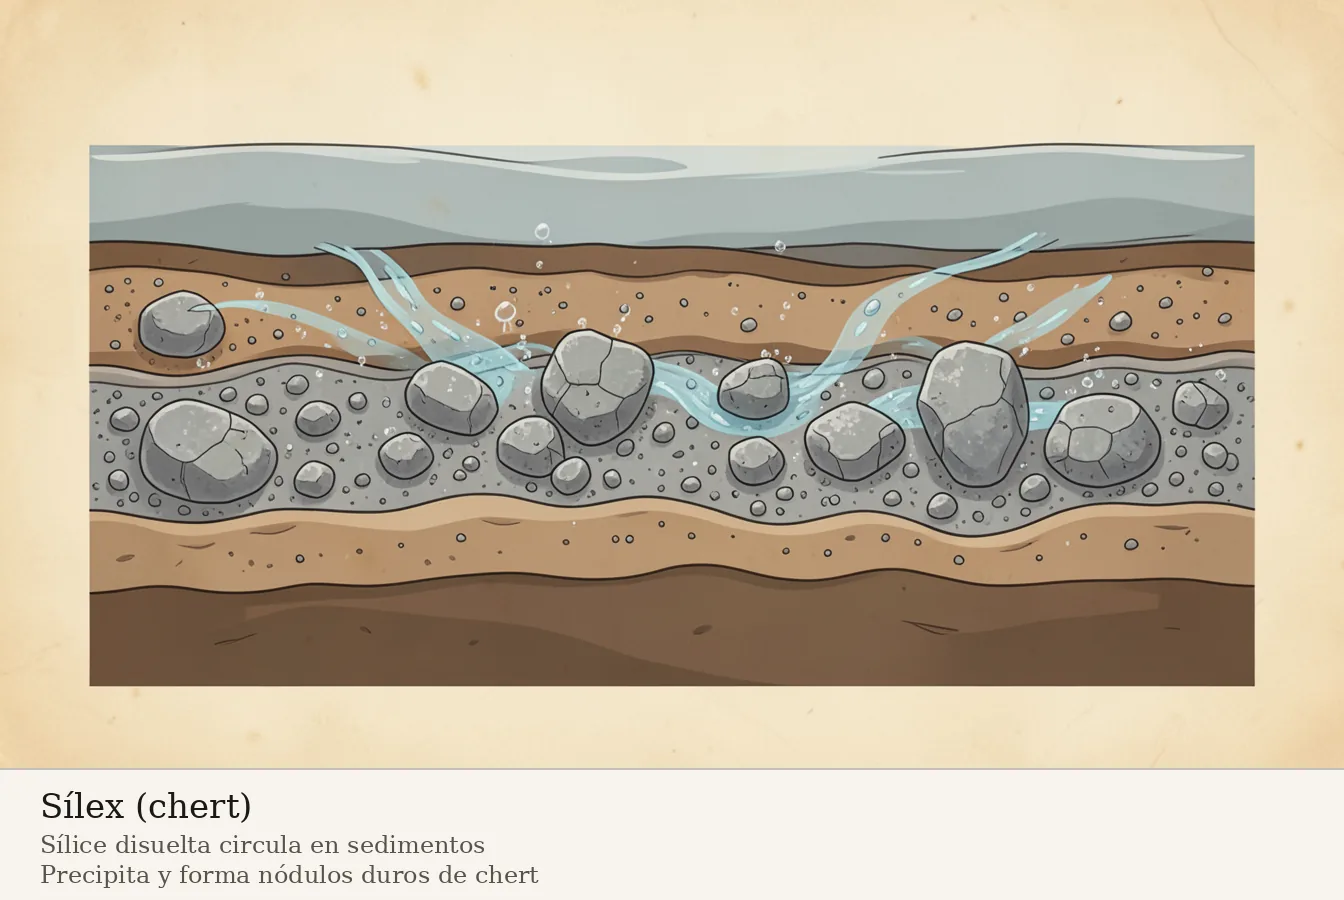
\includegraphics[width=\linewidth]{assets/images/chert.png}
  \end{minipage}\hfill
  \begin{minipage}{0.48\linewidth}
    \centering
    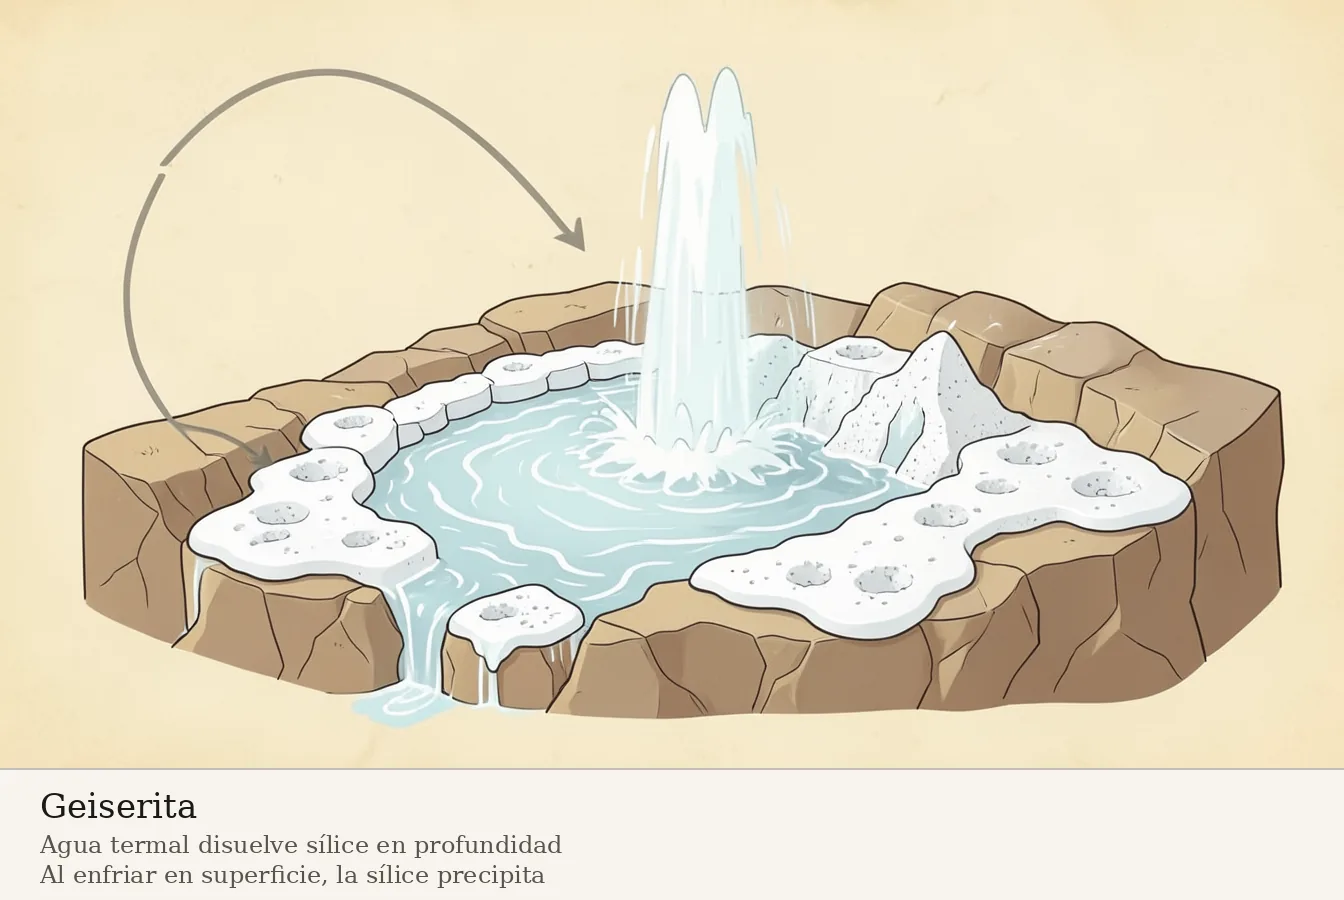
\includegraphics[width=\linewidth]{assets/images/siliceous-sinter.png}
  \end{minipage}
  \caption{Ejemplos de ilustraciones de proceso para clases síliceas}
  \label{fig:siliceas}
\end{figure}

\section{Resultados de la aplicación}

La aplicación Litoteca se encuentra desplegada en Cloudflare Pages:
\url{https://litoteca.pages.dev/}. El repositorio público está en
\url{https://github.com/JheisonMB/litoteca}.

Funcionalidades implementadas:

\begin{table}[H]
  \centering
  \caption{Funcionalidades implementadas en Litoteca}
  \label{tab:funcionalidades}
  \begin{tabular}{@{}p{4.2cm}p{8.2cm}@{}}
    \toprule
    Funcionalidad & Estado \\
    \midrule
    Carga/captura de imagen & Implementada, con validación de tipo y tamaño. \\
    Ficha por clase & Implementada para las 9 clases. \\
    Historial local & Implementado con \texttt{localStorage}. \\
    Mock/galería & Implementado con \texttt{?mock=1} y \texttt{?galeria=1}. \\
    Proxy de predicción & Implementado en \texttt{functions/api/predict.js}. \\
    Guardrail roca/no-roca & Implementado; detector binario antes del clasificador, responde HTTP 422 \texttt{no\_es\_roca}. \\
    Modo sin conexión & Implementado con service worker y mensaje honesto. \\
    Despliegue CF Pages & Implementado con GitHub Actions y Wrangler. \\
    Métricas finales del modelo & Pendientes de la iteración final en Custom Vision. \\
    \bottomrule
  \end{tabular}
\end{table}

\begin{figure}[H]
  \centering
  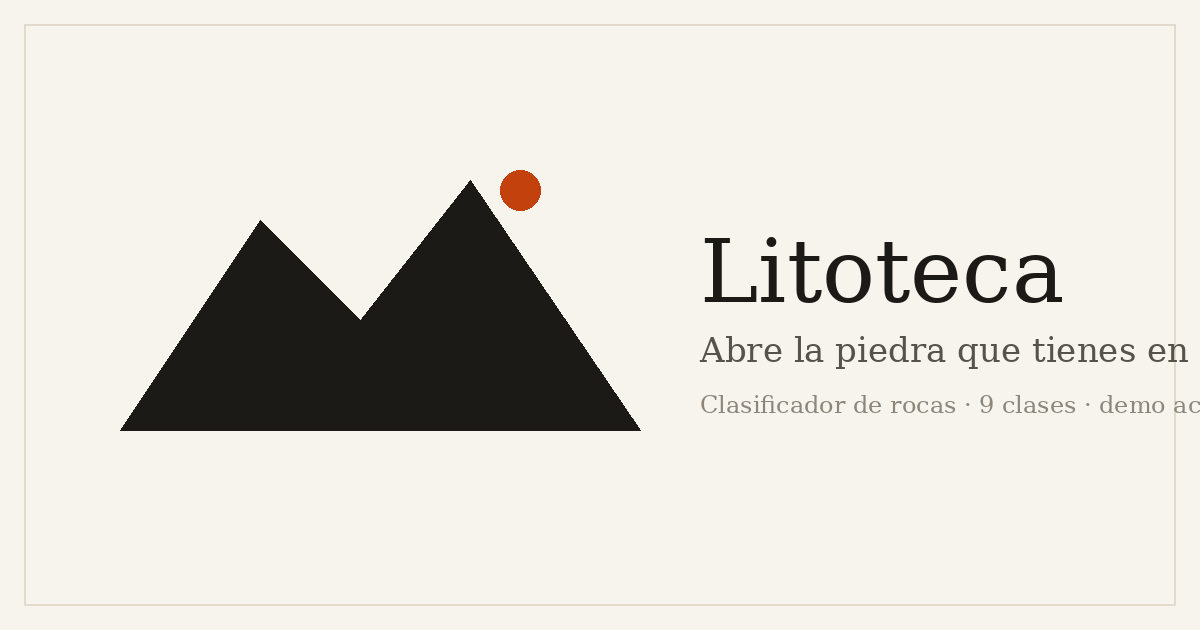
\includegraphics[width=0.75\linewidth]{assets/images/og-image.png}
  \caption{Vista de identidad visual de Litoteca}
  \label{fig:og}
\end{figure}

\section{Resultados del entrenamiento Quick v2}

Se entrenó una segunda iteración Quick en el proyecto limpio
\texttt{litoteca-clean-quick-v2}
(\texttt{8bffd799-5b43-486e-8494-f1174d7ca4e7}, Iteration 1,
\texttt{4792fd31-2f7a-4505-9c72-71c1c3ffe4b8}). El entrenamiento finalizó con
estado \texttt{Completed}, tipo \texttt{Regular}, tiempo de entrenamiento de 9
minutos, y se publicó como \texttt{litoteca-v1} en
\texttt{labunisalle-Prediction}.

\begin{table}[H]
  \centering
  \caption{Comparación global entre iteraciones Quick}
  \label{tab:metricas-globales}
  \begin{tabular}{@{}lrrr@{}}
    \toprule
    Iteración & Precision & Recall & AP \\
    \midrule
    Quick v1 (6276ca2b) & 83.08\% & 52.43\% & 72.74\% \\
    Quick v2 (4792fd31) & 84.88\% & 54.48\% & 77.77\% \\
    \bottomrule
  \end{tabular}
\end{table}

\begin{table}[H]
  \centering
  \caption{Métricas por clase de Quick v2}
  \label{tab:metricas-clase}
  \begin{tabular}{@{}lrrr@{}}
    \toprule
    Clase & Precision & Recall & AP \\
    \midrule
    basalt & 79.31\% & 69.70\% & 85.43\% \\
    chert & 85.71\% & 38.71\% & 73.81\% \\
    clay & 90.00\% & 30.00\% & 64.94\% \\
    conglomerate & 100.00\% & 77.42\% & 93.16\% \\
    diatomite & 76.19\% & 59.26\% & 69.36\% \\
    gypsum & 89.47\% & 54.84\% & 78.59\% \\
    olivine-basalt & 91.30\% & 75.00\% & 92.49\% \\
    shale & 63.64\% & 22.58\% & 58.42\% \\
    siliceous-sinter & 80.95\% & 65.38\% & 78.43\% \\
    \bottomrule
  \end{tabular}
\end{table}

Quick v2 mejora las métricas globales respecto a Quick v1, especialmente en AP.
El desempeño sigue siendo fuerte en \emph{conglomerate}, \emph{olivine-basalt},
\emph{basalt} y \emph{gypsum}, mientras que \emph{shale}, \emph{clay} y
\emph{chert} mantienen recall bajo, coherente con la similitud visual entre clases
síliceas y arcillosas documentada en la preparación del dataset.

\section{Resultados del detector roca/no-roca}

Para evitar que el clasificador multiclase fuerce una etiqueta geológica sobre
imágenes fuera de dominio, se entrenó y publicó un detector binario en Custom
Vision. El dataset \texttt{data/rock-detector} contiene 150 imágenes de
\texttt{rock} y 150 de \texttt{not\_rock}. La iteración
\texttt{2d92f618-115e-4a73-a9ed-006002782c7c} del proyecto
\texttt{2dc1aedb-f66c-4fb1-abc5-54c253440052} se publicó como
\texttt{litoteca-detector-v1} en \texttt{labunisalle-Prediction}.

\begin{table}[H]
  \centering
  \caption{Métricas del detector roca/no-roca}
  \label{tab:detector-metricas}
  \begin{tabular}{@{}lrrr@{}}
    \toprule
    Etiqueta / Global & Precision & Recall & AP \\
    \midrule
    not\_rock & 100.00\% & 100.00\% & --- \\
    rock & 100.00\% & 96.70\% & --- \\
    \midrule
    \textbf{Global} & \textbf{100.00\%} & \textbf{98.28\%} & \textbf{99.97\%} \\
    \bottomrule
  \end{tabular}
\end{table}

En producción, la Function consulta el detector antes del clasificador. Cuando la
imagen se clasifica como \texttt{not\_rock} o la probabilidad de \texttt{rock}
es menor que 0.5, la API responde HTTP 422 con código \texttt{no\_es\_roca} y el
mensaje ``No identificamos una roca en la imagen''. Esta verificación se confirmó
con una imagen no-roca en \url{https://litoteca.pages.dev/}.

\section{Plan de mejora y validación para demo}

Quick v2 ya fue publicado como \texttt{litoteca-v1} y conectado a la Function de
Cloudflare Pages, actualizando \texttt{CUSTOM\_VISION\_PROJECT} al proyecto
\texttt{litoteca-clean-quick-v2}. Como mejora siguiente, se puede lanzar una
iteración Advanced o ajustar el dataset para subir el recall en clases difíciles
(\emph{shale}, \emph{clay}, \emph{chert}); si mejora, se republica sin cambiar el
contrato de la API.

La validación se plantea en dos niveles:

\begin{enumerate}
  \item \textbf{Prueba sintética por API}: ejecutar predicciones sobre imágenes del
        conjunto \texttt{test} limpio ya disponible en \texttt{data/prepared-clean-train/test},
        registrar etiqueta esperada, predicción top-1, confianza y aciertos/errores.
        Esto da evidencia reproducible aunque la evaluación no sea en campo.
  \item \textbf{Prueba de campo para demo}: usar fotos reales tomadas con celular en
        condiciones controladas (buena luz, fondo simple, roca centrada) para mostrar
        el flujo completo de la aplicación. Dado el contexto de la entrega, el foco
        de la demo es la integración funcional y la explicación de resultados, no una
        pericia geológica experta.
\end{enumerate}

Las métricas complementarias solicitadas (F1-score, curva ROC y AUC) se pueden
calcular sobre los resultados de prueba por API/exportación de predicciones, además
de las métricas nativas reportadas por Custom Vision.

\section{Validación sintética por API}

Se repitió la validación sintética contra la iteración publicada actualmente como
\texttt{litoteca-v1} (Quick v2, \texttt{4792fd31-2f7a-4505-9c72-71c1c3ffe4b8}) usando
el conjunto \texttt{data/prepared-clean-train/test} (146 imágenes, una por cluster,
sin fuga). La llamada se realizó al endpoint de predicción de Custom Vision con el
mismo contrato que consume la aplicación.

\begin{table}[H]
  \centering
  \caption{Resultado de validación sintética por API (test limpio, Quick v2)}
  \label{tab:api-test}
  \begin{tabular}{@{}lrrr@{}}
    \toprule
    Clase & Aciertos & Total & Accuracy \\
    \midrule
    basalt & 14 & 15 & 93.33\% \\
    chert & 9 & 14 & 64.29\% \\
    clay & 5 & 12 & 41.67\% \\
    conglomerate & 6 & 13 & 46.15\% \\
    diatomite & 12 & 19 & 63.16\% \\
    gypsum & 18 & 23 & 78.26\% \\
    olivine-basalt & 17 & 19 & 89.47\% \\
    shale & 13 & 20 & 65.00\% \\
    siliceous-sinter & 7 & 11 & 63.64\% \\
    \midrule
    \textbf{Total} & \textbf{101} & \textbf{146} & \textbf{69.18\%} \\
    \bottomrule
  \end{tabular}
\end{table}

Frente a Quick v1 (95/146, 65.07\%), Quick v2 mejora en +6 aciertos (+4.11 puntos
porcentuales). Los errores más frecuentes siguen concentrados en clases visualmente
cercanas: conglomerate$\rightarrow$clay (4), diatomite$\rightarrow$chert (3),
chert$\rightarrow$clay (2), clay$\rightarrow$shale (2),
conglomerate$\rightarrow$siliceous-sinter (2), diatomite$\rightarrow$clay (2),
shale$\rightarrow$diatomite (2), shale$\rightarrow$basalt (2) y
siliceous-sinter$\rightarrow$shale (2).
